% answers.tex —— 2005 年·普通高等学校招生考试·辽宁卷 · 参考答案与详细解析片段
% 由 tools/generate_projects.py 依来源总账自 2005/2005_数学真题_辽宁_试题.md + 2005/2005_数学真题_辽宁_解析正文.md + 2005/2005_数学真题_辽宁_答案要点.md 生成，勿手改（改源 MD 后重跑）

\begin{gktip}
说明：本卷固定来源 PDF 不含官方答案页，以下全部解答为\textbf{独立推导、非官方答案}。选择题给出判定依据，填空题给出完整推导，解答题按印面分值组织步骤。
\end{gktip}

\gkpart{一、选择题}

\begin{answer}
\gksolhead{1}{}

\textbf{题目}：

复数 $z = \dfrac{-1+\mathrm{i}}{1+\mathrm{i}} - 1$ 在复平面内，$z$ 所对应的点在\mbox{（　　）}

\begin{gkopts}(4)
\task A．第一象限
\task B．第二象限
\task C．第三象限
\task D．第四象限
\end{gkopts}

\Needspace{4\baselineskip}
\textbf{解析}

【答案】B

【思路】先化简 $z$。

\Needspace{5\baselineskip}
【详解】因为
\nopagebreak[4]
\[
\frac{-1+\mathrm{i}}{1+\mathrm{i}} = \frac{(-1+\mathrm{i})(1-\mathrm{i})}{(1+\mathrm{i})(1-\mathrm{i})} = \frac{-1+\mathrm{i}+\mathrm{i}-\mathrm{i}^2}{2} = \frac{2\mathrm{i}}{2} = \mathrm{i},
\]
所以 $z = \mathrm{i} - 1 = -1 + \mathrm{i}$，对应点 $(-1, 1)$ 位于第二象限。

\gkanswer{答案：B。}

\end{answer}
\begin{answer}
\gksolhead{2}{}

\textbf{题目}：

极限 $\lim\limits_{x \to x_0} f(x)$ 存在是函数 $f(x)$ 在点 $x = x_0$ 处连续的\mbox{（　　）}

\begin{gkopts}(2)
\task A．充分而不必要的条件
\task B．必要而不充分的条件
\task C．充要条件
\task D．既不充分也不必要的条件
\end{gkopts}

\Needspace{4\baselineskip}
\textbf{解析}

【答案】B

【思路】比较连续与极限存在的定义。

【详解】$f(x)$ 在 $x_0$ 处连续意味着 $\lim\limits_{x \to x_0} f(x) = f(x_0)$，这本身已包含极限存在，故极限存在是连续的必要条件；反之取 $f(x) = \dfrac{x^2-1}{x-1}$（$x \neq 1$）、$f(1) = 0$，则 $\lim\limits_{x \to 1} f(x) = 2$ 存在而 $f(1) \neq 2$，$f$ 在 $x = 1$ 处不连续。故为必要而不充分条件。

\gkanswer{答案：B。}

\end{answer}
\begin{answer}
\gksolhead{3}{}

\textbf{题目}：

设袋中有 80 个红球，20 个白球，若从袋中任取 10 个球，则其中恰有 6 个红球的概率为\mbox{（　　）}

\begin{gkopts}(1)
\task A．$\dfrac{\mathrm{C}_{80}^{4} \cdot \mathrm{C}_{10}^{6}}{\mathrm{C}_{100}^{10}}$
\task B．$\dfrac{\mathrm{C}_{80}^{6} \cdot \mathrm{C}_{10}^{4}}{\mathrm{C}_{100}^{10}}$
\task C．$\dfrac{\mathrm{C}_{80}^{4} \cdot \mathrm{C}_{20}^{6}}{\mathrm{C}_{100}^{10}}$
\task D．$\dfrac{\mathrm{C}_{80}^{6} \cdot \mathrm{C}_{20}^{4}}{\mathrm{C}_{100}^{10}}$
\end{gkopts}

\Needspace{4\baselineskip}
\textbf{解析}

【答案】D

【思路】超几何分布。

\Needspace{5\baselineskip}
【详解】从 100 个球中任取 10 个共有 $\mathrm{C}_{100}^{10}$ 种等可能取法；恰有 6 个红球即从 80 个红球中取 6 个、从 20 个白球中取 4 个，共 $\mathrm{C}_{80}^{6}\mathrm{C}_{20}^{4}$ 种。故所求概率为
\nopagebreak[4]
\[
P = \frac{\mathrm{C}_{80}^{6}\mathrm{C}_{20}^{4}}{\mathrm{C}_{100}^{10}}.
\]

\gkanswer{答案：D。}

\end{answer}
\begin{answer}
\gksolhead{4}{}

\textbf{题目}：

已知 $m$、$n$ 是两条不重合的直线，$\alpha$、$\beta$、$\gamma$ 是三个两两不重合的平面，给出下列四个命题：
① 若 $m \perp \alpha$，$m \perp \beta$，则 $\alpha \parallel \beta$；
② 若 $\alpha \perp \gamma$，$\beta \perp \alpha$，则 $\alpha \parallel \beta$；
③ 若 $m \subset \alpha$，$n \subset \beta$，$m \parallel n$，则 $\alpha \parallel \beta$；
④ 若 $m$、$n$ 是异面直线，$m \subset \alpha$，$m \parallel \beta$，$n \subset \beta$，$n \parallel \alpha$，则 $\alpha \parallel \beta$．
其中真命题是\mbox{（　　）}

\begin{gkopts}(4)
\task A．①和②
\task B．①和③
\task C．③和④
\task D．①和④
\end{gkopts}

\Needspace{4\baselineskip}
\textbf{解析}

【答案】D

【思路】逐条判断，假命题给出反例。

【详解】① 垂直于同一直线的两个平面平行，真命题。② 由 $\alpha \perp \gamma$、$\beta \perp \gamma$ 只能得 $\alpha$、$\beta$ 均垂直于 $\gamma$，它们仍可能相交（如两面墙同垂直于地面），需改成 $\beta \perp \gamma$ 才是真命题，故按印面不是必然结论。③ 两平面内各有一条直线平行，两平面仍可能相交（如 $\alpha \cap \beta = l$ 且 $m \parallel n \parallel l$），假。④ 由 $m \subset \alpha$、$m \parallel \beta$ 知 $\alpha$、$\beta$ 无公共点或 $\alpha \parallel \beta$；若 $\alpha$、$\beta$ 相交于 $l$，则 $m \parallel l$，同理 $n \parallel l$，从而 $m \parallel n$，与 $m$、$n$ 异面矛盾，故 $\alpha \parallel \beta$，真命题。

故选①和④。

\gkanswer{答案：D。}

\end{answer}
\begin{answer}
\gksolhead{5}{}

\textbf{题目}：

函数 $y = \ln\left(x + \sqrt{x^2+1}\right)$ 的反函数是\mbox{（　　）}

\begin{gkopts}(1)
\task A．$y = \dfrac{\mathrm{e}^x + \mathrm{e}^{-x}}{2}$
\task B．$y = -\dfrac{\mathrm{e}^x + \mathrm{e}^{-x}}{2}$
\task C．$y = \dfrac{\mathrm{e}^x - \mathrm{e}^{-x}}{2}$
\task D．$y = -\dfrac{\mathrm{e}^x - \mathrm{e}^{-x}}{2}$
\end{gkopts}

\Needspace{4\baselineskip}
\textbf{解析}

【答案】C

【思路】先解出 $x$，再用 $y$ 表示。

\Needspace{5\baselineskip}
【详解】由 $y = \ln\left(x+\sqrt{x^2+1}\right)$ 得 $\mathrm{e}^y = x + \sqrt{x^2+1}$，又 $\dfrac{1}{\mathrm{e}^y} = \sqrt{x^2+1} - x$，两式相减得
\nopagebreak[4]
\[
x = \frac{\mathrm{e}^y - \mathrm{e}^{-y}}{2}.
\]
交换 $x$、$y$ 得反函数 $y = \dfrac{\mathrm{e}^x - \mathrm{e}^{-x}}{2}$（注意原函数的值域为 $\mathbf{R}$，故定义域为 $\mathbf{R}$）。

\gkanswer{答案：C。}

\end{answer}
\begin{answer}
\gksolhead{6}{}

\textbf{题目}：

若 $\log_{2a}\dfrac{1+a^2}{1+a} < 0$，则 $a$ 的取值范围是\mbox{（　　）}

\begin{gkopts}(2)
\task A．$\left(\dfrac{1}{2}, +\infty\right)$
\task B．$(1, +\infty)$
\task C．$\left(\dfrac{1}{2}, 1\right)$
\task D．$\left(0, \dfrac{1}{2}\right)$
\end{gkopts}

\Needspace{4\baselineskip}
\textbf{解析}

【答案】C

【思路】按底数大于 1、小于 1 分类。

【详解】需 $2a > 0$ 且 $2a \neq 1$。记真数 $t = \dfrac{1+a^2}{1+a}$，则 $t - 1 = \dfrac{a^2-a}{1+a}$，故当 $0 < a < 1$ 时 $t < 1$，当 $a > 1$ 时 $t > 1$。

若 $a > \dfrac{1}{2}$，则底数 $2a > 1$，$\log_{2a} t < 0 \iff 0 < t < 1 \iff 0 < a < 1$，得 $\dfrac{1}{2} < a < 1$。

若 $0 < a < \dfrac{1}{2}$，则底数 $2a < 1$，$\log_{2a} t < 0 \iff t > 1 \iff a > 1$，无解。

故 $a \in \left(\dfrac{1}{2}, 1\right)$。

\gkanswer{答案：C。}

\end{answer}
\begin{answer}
\gksolhead{7}{}

\textbf{题目}：

在 $\mathbf{R}$ 上定义运算 $\otimes$：$x \otimes y = x(1-y)$．若不等式 $(x-a) \otimes (x+a) < 1$ 对任意实数 $x$ 成立，则\mbox{（　　）}

\begin{gkopts}(2)
\task A．$-1 < a < 1$
\task B．$0 < a < 2$
\task C．$-\dfrac{1}{2} < a < \dfrac{3}{2}$
\task D．$-\dfrac{3}{2} < a < \dfrac{1}{2}$
\end{gkopts}

\Needspace{4\baselineskip}
\textbf{解析}

【答案】C

【思路】按定义展开，化为二次不等式恒成立。

\Needspace{5\baselineskip}
【详解】由定义
\nopagebreak[4]
\[
(x-a) \otimes (x+a) = (x-a)\left[1-(x+a)\right] = -x^2 + x - a + a^2.
\]
\Needspace{5\baselineskip}
不等式 $-x^2+x-a+a^2 < 1$ 对任意 $x$ 成立，等价于 $x^2 - x + (1+a-a^2) > 0$ 恒成立，即
\nopagebreak[4]
\[
\Delta = 1 - 4(1+a-a^2) < 0 \iff 4a^2 - 4a - 3 < 0 \iff (2a-3)(2a+1) < 0,
\]
解得 $-\dfrac{1}{2} < a < \dfrac{3}{2}$。

\gkanswer{答案：C。}

\end{answer}
\begin{answer}
\gksolhead{8}{}

\textbf{题目}：

若钝角三角形三内角的度数成等差数列，且最大边长与最小边长的比值为 $m$，则 $m$ 的范围是\mbox{（　　）}

\begin{gkopts}(4)
\task A．$(1, 2)$
\task B．$(2, +\infty)$
\task C．$[3, +\infty)$
\task D．$(3, +\infty)$
\end{gkopts}

\Needspace{4\baselineskip}
\textbf{解析}

【答案】B

【思路】三内角成等差数列确定中间角为 $60^\circ$。

【详解】设三内角从小到大为 $A < B < C$，成等差数列则 $2B = A + C = 180^\circ - B$，故 $B = 60^\circ$，且 $A + C = 120^\circ$。三角形为钝角三角形，故最大角 $C \in (90^\circ, 120^\circ)$，从而 $A = 120^\circ - C \in (0^\circ, 30^\circ)$。

\Needspace{5\baselineskip}
由正弦定理，最大边与最小边之比
\nopagebreak[4]
\[
m = \frac{\sin C}{\sin A} = \frac{\sin C}{\sin(120^\circ - C)},\qquad C \in (90^\circ, 120^\circ).
\]
该函数在 $(90^\circ, 120^\circ)$ 上单调递增：$C \to 90^\circ{}+$ 时 $m \to \dfrac{1}{1/2} = 2$；$C \to 120^\circ{}-$ 时 $\sin A \to 0^+$，$m \to +\infty$。故 $m \in (2, +\infty)$。

\gkanswer{答案：B。}

\end{answer}
\begin{answer}
\gksolhead{9}{}

\textbf{题目}：

若直线 $2x - y + c = 0$ 按向量 $\vec{a} = (1, -1)$ 平移后与圆 $x^2 + y^2 = 5$ 相切，则 $c$ 的值为\mbox{（　　）}

\begin{gkopts}(2)
\task A．$8$ 或 $-2$
\task B．$6$ 或 $-4$
\task C．$4$ 或 $-6$
\task D．$2$ 或 $-8$
\end{gkopts}

\Needspace{4\baselineskip}
\textbf{解析}

【答案】A

【思路】先求平移后的直线，再用圆心到直线的距离等于半径。

\Needspace{5\baselineskip}
【详解】直线 $2x-y+c = 0$ 按向量 $\vec{a} = (1,-1)$ 平移，即把 $x$ 换成 $x-1$、$y$ 换成 $y+1$，得
\nopagebreak[4]
\[
2(x-1) - (y+1) + c = 0,\quad\text{\text{即}}\quad 2x - y + (c-3) = 0.
\]
\Needspace{5\baselineskip}
该直线与圆 $x^2+y^2 = 5$ 相切，故圆心到它的距离
\nopagebreak[4]
\[
\frac{|c-3|}{\sqrt{2^2+(-1)^2}} = \sqrt{5} \iff |c-3| = 5,
\]
解得 $c = 8$ 或 $c = -2$。

\gkanswer{答案：A。}

\end{answer}
\begin{answer}
\gksolhead{10}{}

\textbf{题目}：

已知 $y = f(x)$ 是定义在 $\mathbf{R}$ 上的单调函数，实数 $x_1 \neq x_2$，$\lambda \neq -1$，$\alpha = \dfrac{x_1 + \lambda x_2}{1+\lambda}$，$\beta = \dfrac{x_2 + \lambda x_1}{1+\lambda}$．若 $|f(x_1) - f(x_2)| < |f(\alpha) - f(\beta)|$，则\mbox{（　　）}

\begin{gkopts}(2)
\task A．$\lambda < 0$
\task B．$\lambda = 0$
\task C．$0 < \lambda < 1$
\task D．$\lambda \geqslant 1$
\end{gkopts}

\Needspace{4\baselineskip}
\textbf{解析}

【答案】A

【思路】先比较 $\alpha$、$\beta$ 与 $x_1$、$x_2$ 的位置关系，再用单调性。

\Needspace{5\baselineskip}
【详解】因为
\nopagebreak[4]
\[
\alpha - \beta = \frac{x_1 + \lambda x_2 - x_2 - \lambda x_1}{1+\lambda} = \frac{(1-\lambda)(x_1-x_2)}{1+\lambda},
\]
所以 $|\alpha - \beta| = |x_1 - x_2| \cdot \dfrac{|1-\lambda|}{|1+\lambda|}$。

\Needspace{5\baselineskip}
$f$ 在 $\mathbf{R}$ 上单调，故对任意 $u$、$v$，$|f(u)-f(v)|$ 随 $|u-v|$ 严格增大。由 $|f(x_1)-f(x_2)| < |f(\alpha)-f(\beta)|$ 得
\nopagebreak[4]
\[
|x_1 - x_2| < |\alpha - \beta| \iff \frac{|1-\lambda|}{|1+\lambda|} > 1 \iff (1-\lambda)^2 > (1+\lambda)^2 \iff \lambda < 0.
\]
（$\lambda \neq -1$ 已在题设中排除。）

\gkanswer{答案：A。}

\end{answer}
\begin{answer}
\gksolhead{11}{}

\textbf{题目}：

已知双曲线的中心在原点，离心率为 $\sqrt{3}$．若它的一条准线与抛物线 $y^2 = 4x$ 的准线重合，则该双曲线与抛物线 $y^2 = 4x$ 的交点到原点的距离是\mbox{（　　）}

\begin{gkopts}(2)
\task A．$2\sqrt{3} + \sqrt{6}$
\task B．$\sqrt{21}$
\task C．$\sqrt{18 + 12\sqrt{2}}$
\task D．$21$
\end{gkopts}

\Needspace{4\baselineskip}
\textbf{解析}

【答案】B

【思路】由准线重合与离心率定出 $a$、$b$、$c$，再求交点。

【详解】抛物线 $y^2 = 4x$ 的准线为 $x = -1$。双曲线中心在原点、焦点在 $x$ 轴上（准线为竖直线），其左准线为 $x = -\dfrac{a^2}{c}$，故 $\dfrac{a^2}{c} = 1$，即 $a^2 = c$。

又 $e = \dfrac{c}{a} = \sqrt{3}$，得 $c = \sqrt{3}a$，代入 $a^2 = c$ 得 $a = \sqrt{3}$，$c = 3$，$b^2 = c^2 - a^2 = 6$。双曲线方程为 $\dfrac{x^2}{3} - \dfrac{y^2}{6} = 1$。

与 $y^2 = 4x$ 联立得 $\dfrac{x^2}{3} - \dfrac{4x}{6} = 1$，即 $x^2 - 2x - 3 = 0$，解得 $x = 3$（$x = -1$ 舍去），$y^2 = 12$。交点与原点距离为 $\sqrt{3^2 + 12} = \sqrt{21}$。

\gkanswer{答案：B。}

\end{answer}
\begin{answer}
\gksolhead{12}{}

\textbf{题目}：

一给定函数 $y = f(x)$ 的图象在下列图中，并且对任意 $a_1 \in (0, 1)$，由关系式 $a_{n+1} = f(a_n)$ 得到的数列 $\{a_n\}$ 满足 $a_{n+1} > a_n$（$n \in \mathbf{N}^*$），则该函数的图象是\mbox{（　　）}
\nopagebreak[4]
\begin{center}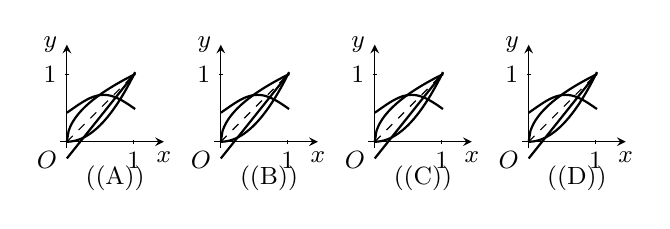
\begin{tikzpicture}[>=stealth, scale=0.85]
  % 四个候选图象：均画在 (0,1) 上，虚线为 y=x
  \foreach \dx/\name/\kind in {0/(A)/above, 2.3/(B)/below, 4.6/(C)/crossover, 6.9/(D)/crossunder}{
    \begin{scope}[shift={(\dx,0)}]
      \draw[->] (-0.1,0) -- (1.45,0) node[below] {\small $x$};
      \draw[->] (0,-0.1) -- (0,1.45) node[left] {\small $y$};
      \node[below left] at (0,0) {\small $O$};
      \draw[dashed] (0,0) -- (1.05,1.05);
      \draw (-0.03,1) -- (0.03,1) node[left=1pt] {\small $1$};
      \draw (1,-0.03) -- (1,0.03) node[below=1pt] {\small $1$};
      \ifthenelse{\equal{\kind}{above}}{%
        \draw[thick, domain=0:1.02, samples=40] plot (\x,{sqrt(\x)});%
      }{%
      \ifthenelse{\equal{\kind}{below}}{%
        \draw[thick, domain=0:1.02, samples=40] plot (\x,{\x*\x});%
      }{%
      \ifthenelse{\equal{\kind}{crossover}}{%
        \draw[thick, domain=0:1.02, samples=40] plot (\x,{1.25*\x - 0.25});%
      }{%
        \draw[thick, domain=0:1.02, samples=40] plot (\x,{0.55*exp(-2.2*(\x-0.55)^2)+0.15});%
      }}}%
      \node[below] at (0.72,-0.22) {\small (\name)};
    \end{scope}
  }
\end{tikzpicture}
\end{center}
\nopagebreak[4]
\begin{gkopts}(4)
\task A．图（A）
\task B．图（B）
\task C．图（C）
\task D．图（D）
\end{gkopts}

\Needspace{4\baselineskip}
\textbf{解析}

【答案】A

【思路】$a_{n+1} > a_n$ 要求递推函数的图象位于直线 $y = x$ 上方（在 $(0,1)$ 上）。

【详解】若 $f$ 的图象在区间 $(0,1)$ 上位于直线 $y = x$ 上方，即 $f(x) > x$，则对任意 $a_1 \in (0,1)$ 都有 $a_2 = f(a_1) > a_1$，且同样 $a_{n+1} = f(a_n) > a_n$，满足题意。图（A）即为这种情形；图（B）在 $(0,1)$ 上位于 $y = x$ 下方（数列递减），图（C）（D）与 $y = x$ 相交（数列会穿越不动点，不能对一切 $a_1 \in (0,1)$ 单调递增）。

\gkanswer{答案：A。}

\end{answer}
\gkpart{二、填空题}

\begin{answer}
\gksolhead{13}{}

\textbf{题目}：

$\left(x^{\frac{1}{2}} - 2x^{-\frac{1}{2}}\right)^{n}$ 的展开式中常数项是 $\underline{\hspace{2cm}}$．

\Needspace{4\baselineskip}
\textbf{解析}

【答案】当 $n$ 为偶数时为 $\mathrm{C}_{n}^{\frac{n}{2}}(-2)^{\frac{n}{2}}$；当 $n$ 为奇数时展式中不存在常数项

【思路】写出通项，令 $x$ 的指数为零。

\Needspace{5\baselineskip}
【详解】展开式通项
\nopagebreak[4]
\[
T_{k+1} = \mathrm{C}_{n}^{k}\left(x^{\frac{1}{2}}\right)^{n-k}\left(-2x^{-\frac{1}{2}}\right)^{k} = \mathrm{C}_{n}^{k}(-2)^{k}x^{\frac{n-2k}{2}},\qquad k = 0,1,\dots,n.
\]
常数项要求 $\dfrac{n-2k}{2} = 0$，即 $k = \dfrac{n}{2}$。故当 $n$ 为偶数时常数项为 $\mathrm{C}_{n}^{\frac{n}{2}}(-2)^{\frac{n}{2}}$；当 $n$ 为奇数时 $k$ 不是整数，不存在常数项。

（印面指数为字母 $n$，此处按固定源字面作答。若按通行版本取 $n = 6$，则常数项为 $\mathrm{C}_{6}^{3}(-2)^{3} = -160$。）

\gkanswer{答案：$n$ 为偶数时常数项为 $\mathrm{C}_{n}^{\frac{n}{2}}(-2)^{\frac{n}{2}}$；$n$ 为奇数时展开式中不存在常数项。}

\end{answer}
\begin{answer}
\gksolhead{14}{}

\textbf{题目}：

如图，正方体的棱长为 $1$，$C$、$D$ 分别是两条棱的中点，$A$、$B$、$M$ 是顶点，那么点 $M$ 到截面 $ABCD$ 的距离是 $\underline{\hspace{2cm}}$．
\nopagebreak[4]
\begin{center}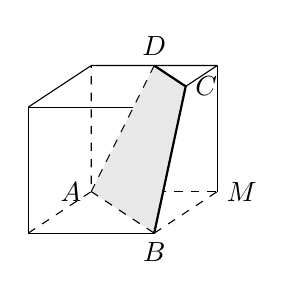
\begin{tikzpicture}[>=stealth, scale=1.6, line join=round]
  % 投影：x 向右、y 向右上（景深）、z 向上
  \def\px#1#2#3{#1+0.5*#2}
  \def\py#1#2#3{#3+0.33*#2}
  % 立方体八个顶点
  \coordinate (FBL) at (0,0);
  \coordinate (BBL) at (0.5,0.33);   % A
  \coordinate (FBR) at (1,0);        % B
  \coordinate (BBR) at (1.5,0.33);   % M
  \coordinate (FTL) at (0,1);
  \coordinate (BTL) at (0.5,1.33);
  \coordinate (FTR) at (1,1);
  \coordinate (BTR) at (1.5,1.33);
  % 可见棱（实线）
  \draw (FBL)--(FBR)--(FTR)--(FTL)--cycle;
  \draw (FTL)--(BTL)--(BTR)--(FTR);
  \draw (BTR)--(BBR);
  % 不可见棱（虚线）
  \draw[dashed] (FBL)--(BBL)--(BTL);
  \draw[dashed] (BBL)--(BBR);
  \draw[dashed] (FBR)--(BBR);
  % 截面：C、D 为两条棱中点，A、B、M 为顶点
  \coordinate (C) at (1.25,1.165);
  \coordinate (D) at (1.0,1.33);
  \fill[gray!18] (0.5,0.33)--(1,0)--(1.25,1.165)--(1.0,1.33)--cycle;
  \draw[dashed] (0.5,0.33)--(1,0);
  \draw[dashed] (0.5,0.33)--(1.0,1.33);
  \draw[thick] (1,0)--(1.25,1.165)--(1.0,1.33);
  % 标注
  \node[left] at (0.5,0.33) {$A$};
  \node[below] at (1,0) {$B$};
  \node[right] at (1.5,0.33) {$M$};
  \node[right] at (1.25,1.165) {$C$};
  \node[above] at (1.0,1.33) {$D$};
\end{tikzpicture}
\end{center}
\nopagebreak[4]
\Needspace{4\baselineskip}
\textbf{解析}

【答案】$\dfrac{2}{3}$

【思路】建立坐标系求截面方程，再算点到平面距离。

\Needspace{5\baselineskip}
【详解】设 $M$ 为正方体一个顶点，$A$、$B$ 是与 $M$ 相邻的两个顶点。以 $M$ 为原点、三条棱为坐标轴建立空间直角坐标系，取 $A(1,0,0)$、$B(0,1,0)$，则 $C$、$D$ 为过 $M$ 的两条棱的公共端的另两条棱的中点，可设
\nopagebreak[4]
\[
C\left(\frac{1}{2}, 0, 1\right),\qquad D\left(0, \frac{1}{2}, 1\right).
\]
（$C$ 是棱 $(0,0,1)$—$(1,0,1)$ 的中点，$D$ 是棱 $(0,0,1)$—$(0,1,1)$ 的中点。）

\Needspace{5\baselineskip}
设截面 $ABCD$ 的方程为 $x + y + \lambda z = 1$，代入 $C$ 得 $\dfrac{1}{2} + \lambda = 1$，$\lambda = \dfrac{1}{2}$，且 $D$ 也满足该方程，故截面所在平面为
\nopagebreak[4]
\[
x + y + \frac{1}{2}z = 1.
\]
\Needspace{5\baselineskip}
点 $M(0,0,0)$ 到该平面的距离
\nopagebreak[4]
\[
d = \frac{|0+0+0-1|}{\sqrt{1^2+1^2+\left(\frac{1}{2}\right)^2}} = \frac{1}{\frac{3}{2}} = \frac{2}{3}.
\]

\gkanswer{答案：$\dfrac{2}{3}$。}

\end{answer}
\begin{answer}
\gksolhead{15}{}

\textbf{题目}：

用 $1$、$2$、$3$、$4$、$5$、$6$、$7$、$8$ 组成没有重复数字的八位数，要求 $1$ 和 $2$ 相邻，$3$ 与 $4$ 相邻，$5$ 与 $6$ 相邻，而 $7$ 与 $8$ 不相邻，这样的八位数共有 $\underline{\hspace{2cm}}$ 个．（用数字作答）

\Needspace{4\baselineskip}
\textbf{解析}

【答案】$576$

【思路】用相邻捆绑与容斥。

\Needspace{5\baselineskip}
【详解】把 $1$ 与 $2$、$3$ 与 $4$、$5$ 与 $6$ 分别捆成三块，每块内部有 $2$ 种排列，连同 $7$、$8$ 共 $5$ 个"元素"，共有
\nopagebreak[4]
\[
5! \cdot 2^3 = 960
\]
个八位数。

\Needspace{5\baselineskip}
其中 $7$ 与 $8$ 也相邻的情形：把 $7$ 与 $8$ 再捆成一块，共 $4$ 块，每块内部 $2$ 种排列，共
\nopagebreak[4]
\[
4! \cdot 2^4 = 384
\]
个。

故满足条件的八位数共有 $960 - 384 = 576$ 个。

\gkanswer{答案：$576$。}

\end{answer}
\begin{answer}
\gksolhead{16}{}

\textbf{题目}：

$\omega$ 是正实数，设 $S_\omega = \{\theta \mid f(x) = \cos[\omega(x+\theta)] \text{ \text{是奇函数}}\}$，若对每个实数 $a$，$S_\omega \cap (a, a+1)$ 的元素不超过 $2$ 个，且有 $a$ 使 $S_\omega \cap (a, a+1)$ 含 $2$ 个元素，则 $\omega$ 的取值范围是 $\underline{\hspace{2cm}}$．

\Needspace{4\baselineskip}
\textbf{解析}

【答案】$(\pi, 2\pi]$

【思路】先刻画集合 $S_\omega$，再把它化为等距点集在长度为 1 的区间内的计数问题。

\Needspace{5\baselineskip}
【详解】$f(x) = \cos[\omega(x+\theta)] = \cos(\omega x + \omega\theta)$ 为奇函数，要求 $f(0) = 0$ 且 $f(-x) = -f(x)$，即
\nopagebreak[4]
\[
\cos(\omega\theta) = 0 \iff \omega\theta = \frac{\pi}{2} + k\pi\ (k \in \mathbf{Z}).
\]
故 $S_\omega = \left\{\theta \;\middle|\; \theta = \dfrac{\pi/2 + k\pi}{\omega},\ k \in \mathbf{Z}\right\}$ 是公差为 $d = \dfrac{\pi}{\omega}$ 的等差数列。

\Needspace{5\baselineskip}
任意长度为 $1$ 的开区间内至多含 $2$ 个 $S_\omega$ 中的点，等价于 $d \geqslant \dfrac{1}{2}$；存在长度为 $1$ 的开区间恰含 $2$ 个点，等价于 $d < 1$（若 $d \geqslant 1$，任一长度 $1$ 的开区间至多含 $1$ 个点）。于是
\nopagebreak[4]
\[
\frac{1}{2} \leqslant \frac{\pi}{\omega} < 1 \iff \pi < \omega \leqslant 2\pi.
\]

\gkanswer{答案：$(\pi, 2\pi]$。}

\end{answer}
\gkpart{三、解答题}

\begin{answer}
\gksolhead{17}{}

\textbf{题目}：

（本小题满分 12 分）已知三棱锥 $P-ABC$ 中，$E$、$F$ 分别是 $AC$、$AB$ 的中点，$\triangle ABC$、$\triangle PEF$ 都是正三角形，$PF \perp AB$．
\nopagebreak[4]
\begin{center}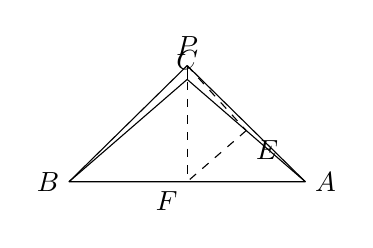
\begin{tikzpicture}[>=stealth, scale=1.5, line join=round]
  % 投影：x 向右，y 向屏幕内（0.5 压缩），z 向上（0.85 压缩）
  \coordinate (A) at (1,0);
  \coordinate (B) at (-1,0);
  \coordinate (C) at (0,0.866);
  \coordinate (F) at (0,0);
  \coordinate (E) at (0.5,0.433);
  \coordinate (P) at (0,0.983);
  % 棱
  \draw (A)--(B)--(C)--cycle;
  \draw (P)--(A);
  \draw (P)--(B);
  \draw (P)--(C);
  % 辅助线（中位线与等边三角形 PEF）
  \draw[dashed] (E)--(F);
  \draw[dashed] (P)--(F);
  \draw[dashed] (P)--(E);
  % 标注
  \node[right] at (A) {$A$};
  \node[left] at (B) {$B$};
  \node[above] at (C) {$C$};
  \node[above] at (P) {$P$};
  \node[below left] at (F) {$F$};
  \node[below right] at (E) {$E$};
\end{tikzpicture}
\end{center}
\nopagebreak[4]
(1) 证明：$PC \perp \text{\text{平面} } PAB$；
(2) 求二面角 $P-AB-C$ 的平面角的余弦值；
(3) 若点 $P$、$A$、$B$、$C$ 在一个表面积为 $12\pi$ 的球面上，求 $\triangle ABC$ 的边长．

\Needspace{4\baselineskip}
\textbf{解析}

【答案】(1) 证明见下；(2) $\dfrac{\sqrt{3}}{3}$；(3) $2\sqrt{2}$

【思路】$F$ 为 $AB$ 中点、$\triangle ABC$ 正三角形给出 $CF \perp AB$，与 $PF \perp AB$ 合成线面垂直；再以 $F$ 为原点建系求二面角与外接球半径。

【详解】设 $\triangle ABC$ 的边长为 $s$（即 $AB = BC = CA = s$）。因为 $F$ 是 $AB$ 的中点，所以 $AF = FB = \dfrac{s}{2}$；又 $E$ 是 $AC$ 的中点，故 $EF$ 是 $\triangle ABC$ 的中位线，$EF = \dfrac{BC}{2} = \dfrac{s}{2}$，且 $EF \parallel BC$。

由 $\triangle PEF$ 是正三角形得 $PE = EF = PF = \dfrac{s}{2}$。

\Needspace{5\baselineskip}
以 $F$ 为原点，$AB$ 所在直线为 $x$ 轴，平面 $ABC$ 为 $xOy$ 平面建立空间直角坐标系，取
\nopagebreak[4]
\[
A\left(\frac{s}{2}, 0, 0\right),\quad B\left(-\frac{s}{2}, 0, 0\right),\quad C\left(0, \frac{\sqrt{3}}{2}s, 0\right),\quad E\left(\frac{s}{4}, \frac{\sqrt{3}}{4}s, 0\right).
\]
\Needspace{5\baselineskip}
设 $P(0, y, z)$。由 $PF \perp AB$ 知 $P$ 在 $x = 0$ 平面上，此即已用。由 $PF = \dfrac{s}{2}$ 得 $y^2 + z^2 = \dfrac{s^2}{4}$；由 $PE = \dfrac{s}{2}$ 得
\nopagebreak[4]
\[
\left(\frac{s}{4}\right)^2 + \left(y - \frac{\sqrt{3}}{4}s\right)^2 + z^2 = \frac{s^2}{4}.
\]
\Needspace{5\baselineskip}
两式相减得 $-\dfrac{\sqrt{3}}{2}sy + \dfrac{3s^2}{16} = -\dfrac{s^2}{16}$，即 $y = \dfrac{\sqrt{3}}{6}s$，从而 $z^2 = \dfrac{s^2}{4} - \dfrac{s^2}{12} = \dfrac{s^2}{6}$，取 $z = \dfrac{s}{\sqrt{6}}$。于是
\nopagebreak[4]
\[
P\left(0, \frac{\sqrt{3}}{6}s, \frac{\sqrt{6}}{6}s\right).
\]

\gksubpart{(1)}

\Needspace{5\baselineskip}
$\overrightarrow{PC} = \left(0, \dfrac{\sqrt{3}}{3}s, -\dfrac{\sqrt{6}}{6}s\right)$，$\overrightarrow{PA} = \left(\dfrac{s}{2}, -\dfrac{\sqrt{3}}{6}s, -\dfrac{\sqrt{6}}{6}s\right)$，而
\nopagebreak[4]
\[
\overrightarrow{PC} \cdot \overrightarrow{PA} = 0 - \frac{3}{18}s^2 + \frac{6}{36}s^2 = -\frac{s^2}{6} + \frac{s^2}{6} = 0,
\]
故 $PC \perp PA$。又 $\overrightarrow{AB} = (-s, 0, 0)$，$\overrightarrow{PC} \cdot \overrightarrow{AB} = 0$，故 $PC \perp AB$。$PA$ 与 $AB$ 相交于 $A$ 且同在平面 $PAB$ 内，所以 $PC \perp$ 平面 $PAB$。

\gksubpart{(2)}

\Needspace{5\baselineskip}
平面 $PAB$ 的法向量可取 $\overrightarrow{PC}$，平面 $ABC$ 的法向量为 $\vec{n} = (0,0,1)$。设二面角 $P-AB-C$ 的平面角为 $\varphi$，则
\nopagebreak[4]
\[
\cos\varphi = \frac{\left|\overrightarrow{PC} \cdot \vec{n}\right|}{\left|\overrightarrow{PC}\right|\left|\vec{n}\right|} = \frac{\frac{\sqrt{6}}{6}s}{\sqrt{\frac{s^2}{3} + \frac{s^2}{6}}} = \frac{\frac{\sqrt{6}}{6}s}{\frac{\sqrt{2}}{2}s} = \frac{\sqrt{3}}{3}.
\]

\gksubpart{(3)}

点 $A$、$B$、$C$ 构成边长 $s$ 的正三角形，其外心为 $G\left(0, \dfrac{\sqrt{3}}{6}s, 0\right)$。球心 $O$ 到 $A$、$B$、$C$ 等距，故 $O$ 在过 $G$ 且垂直于平面 $ABC$ 的直线上，设 $O(0, \dfrac{\sqrt{3}}{6}s, t)$。

\Needspace{5\baselineskip}
于是
\nopagebreak[4]
\[
R^2 = |OA|^2 = |GA|^2 + t^2 = \frac{s^2}{3} + t^2,
\]
\Needspace{5\baselineskip}
又 $P\left(0, \dfrac{\sqrt{3}}{6}s, \dfrac{\sqrt{6}}{6}s\right)$ 与 $O$ 的 $y$ 坐标相同，故 $|OP| = \left|\dfrac{\sqrt{6}}{6}s - t\right|$，由 $|OP| = R$ 得
\nopagebreak[4]
\[
\frac{s^2}{6} - \frac{\sqrt{6}}{3}st + t^2 = \frac{s^2}{3} + t^2 \iff t = -\frac{\sqrt{6}}{12}s.
\]
\Needspace{5\baselineskip}
代回得
\nopagebreak[4]
\[
R^2 = \frac{s^2}{3} + \frac{6}{144}s^2 = \frac{3}{8}s^2.
\]
球的表面积为 $4\pi R^2 = 12\pi$，即 $R^2 = 3$，故 $\dfrac{3}{8}s^2 = 3$，$s^2 = 8$，$s = 2\sqrt{2}$。

即 $\triangle ABC$ 的边长为 $2\sqrt{2}$。

\gkanswer{答案（1）：由 $\overrightarrow{PC}\cdot\overrightarrow{PA}=0$ 得 $PC \perp PA$，又 $PC \perp AB$，故 $PC \perp$ 平面 $PAB$。}

\gkanswer{答案（2）：$\dfrac{\sqrt{3}}{3}$。}

\gkanswer{答案（3）：$2\sqrt{2}$。}

\end{answer}
\begin{answer}
\gksolhead{18}{}

\textbf{题目}：

（本小题满分 12 分）如图，在直径为 $1$ 的圆 $O$ 中，作一关于圆心对称、邻边互相垂直的十字形，其中 $y > x > 0$．
\nopagebreak[4]
\begin{center}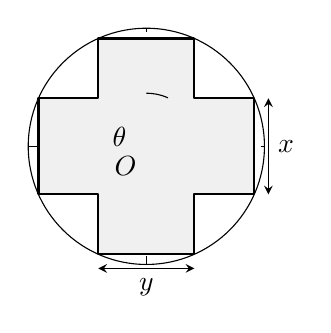
\begin{tikzpicture}[>=stealth, scale=1.5, line join=round]
  \def\th{24}
  \pgfmathsetmacro{\xh}{sin(\th)}
  \pgfmathsetmacro{\yh}{cos(\th)}
  % 圆（直径 1，图中按比例放大）
  \draw (0,0) circle (1);
  \draw[dashed] (-1,0) -- (1,0);
  \draw[dashed] (0,-1) -- (0,1);
  % 十字形
  \draw[thick, fill=gray!12]
    (\yh,\xh) -- (\xh,\xh) -- (\xh,\yh) -- (-\xh,\yh) -- (-\xh,\xh) -- (-\yh,\xh)
    -- (-\yh,-\xh) -- (-\xh,-\xh) -- (-\xh,-\yh) -- (\xh,-\yh) -- (\xh,-\xh) -- (\yh,-\xh) -- cycle;
  % 角 theta
  \draw (0,0.45) arc (90:90-\th:0.45);
  \node at ({0.40*cos(90-\th/2+90)},{0.40*sin(90-\th/2+90)}) [right=1pt] {$\theta$};
  % 尺寸标注
  \draw[<->] (\yh+0.12,-\xh) -- (\yh+0.12,\xh) node[midway,right] {$x$};
  \draw[<->] (-\xh,-\yh-0.12) -- (\xh,-\yh-0.12) node[midway,below] {$y$};
  \node[below left] at (0,0) {$O$};
\end{tikzpicture}
\end{center}
\nopagebreak[4]
(1) 将十字形的面积表示为 $\theta$ 的函数；
(2) $\theta$ 为何值时，十字形的面积最大？最大面积是多少？

\Needspace{4\baselineskip}
\textbf{解析}

【答案】(1) $S(\theta) = \sin 2\theta - \sin^2\theta$，$\theta \in \left(0, \dfrac{\pi}{4}\right)$；(2) 当 $\tan\theta = \dfrac{\sqrt{5}-1}{2}$ 时 $S$ 最大，最大值为 $\dfrac{\sqrt{5}-1}{2}$

【思路】用 $\theta$ 表示十字形的臂厚 $x$ 与臂长 $y$，再用 $\sin\theta$、$\cos\theta$ 表达。

【详解】

\gksubpart{(1)}

\Needspace{5\baselineskip}
设十字形每条臂的宽为 $x$，长为 $y$，其中 $y > x > 0$。十字形的中心是边长为 $x$ 的正方形，四个臂伸出后总面积
\nopagebreak[4]
\[
S = 2xy - x^2.
\]
\Needspace{5\baselineskip}
由题意，十字形的 8 个外顶点都在直径为 $1$（半径为 $\dfrac{1}{2}$）的圆上。在以圆心为原点、以竖直对称轴为始边、$\theta$ 为极角的极坐标系中，第一象限外顶点的坐标为 $\left(\dfrac{x}{2}, \dfrac{y}{2}\right)$，其中极角为 $\theta$，于是
\nopagebreak[4]
\[
\sin\theta = \frac{x/2}{1/2} = x,\qquad \cos\theta = \frac{y/2}{1/2} = y.
\]
\Needspace{5\baselineskip}
由 $y > x > 0$ 得 $0 < \theta < \dfrac{\pi}{4}$。代入面积式得
\nopagebreak[4]
\[
S(\theta) = 2\sin\theta\cos\theta - \sin^2\theta = \sin 2\theta - \sin^2\theta,\qquad \theta \in \left(0, \frac{\pi}{4}\right).
\]

\gksubpart{(2)}

\Needspace{5\baselineskip}
求导：
\nopagebreak[4]
\[
S'(\theta) = 2\cos 2\theta - 2\sin\theta\cos\theta = 2\cos 2\theta - \sin 2\theta.
\]
令 $S'(\theta) = 0$ 得 $\tan 2\theta = 2$。因 $2\theta \in \left(0, \dfrac{\pi}{2}\right)$，故 $\tan 2\theta = 2$ 在区间内有唯一解，且 $\theta$ 由小到大时 $S'$ 由正变负，该点为最大值点。

\Needspace{5\baselineskip}
由 $\tan 2\theta = \dfrac{2\tan\theta}{1-\tan^2\theta} = 2$ 得 $\tan^2\theta + \tan\theta - 1 = 0$，取正根
\nopagebreak[4]
\[
\tan\theta = \frac{\sqrt{5}-1}{2}.
\]
\Needspace{5\baselineskip}
此时用 $\sin 2\theta = \dfrac{2\tan\theta}{1+\tan^2\theta}$、$\sin^2\theta = \dfrac{\tan^2\theta}{1+\tan^2\theta}$ 及 $\tan^2\theta = 1 - \tan\theta$ 化简，或直接用 $\tan 2\theta = 2$ 得 $\sin 2\theta = \dfrac{2}{\sqrt{5}}$、$\cos 2\theta = \dfrac{1}{\sqrt{5}}$，从而
\nopagebreak[4]
\[
S = \sin 2\theta - \frac{1 - \cos 2\theta}{2} = \frac{2}{\sqrt{5}} - \frac{1}{2} + \frac{1}{2\sqrt{5}} = \frac{5}{2\sqrt{5}} - \frac{1}{2} = \frac{\sqrt{5}}{2} - \frac{1}{2} = \frac{\sqrt{5}-1}{2}.
\]
即最大面积为 $\dfrac{\sqrt{5}-1}{2}$。

\gkanswer{答案（1）：$S(\theta)=\sin 2\theta - \sin^{2}\theta$，$\theta \in \left(0, \dfrac{\pi}{4}\right)$。}

\gkanswer{答案（2）：当 $\tan\theta=\dfrac{\sqrt{5}-1}{2}$ 时 $S$ 取最大值 $\dfrac{\sqrt{5}-1}{2}$。}

\end{answer}
\begin{answer}
\gksolhead{19}{}

\textbf{题目}：

（本小题满分 12 分）已知函数 $f(x) = \dfrac{x+3}{x+1}$（$x \neq -1$）．设数列 $\{a_n\}$ 满足 $a_1 = 1$，$a_{n+1} = f(a_n)$，数列 $\{b_n\}$ 满足 $b_n = |a_n - \sqrt{3}|$，$S_n = b_1 + b_2 + \cdots + b_n$（$n \in \mathbf{N}^*$）．

(1) 用数学归纳法证明：$b_n \leqslant \dfrac{(\sqrt{3}-1)^n}{2^{n-1}}$；
(2) 证明：$S_n < \dfrac{2\sqrt{3}}{3}$．

\Needspace{4\baselineskip}
\textbf{解析}

【答案】(1)(2) 证明见下

【思路】先化简 $a_{n+1} - \sqrt{3}$，得到 $b_n$ 的递推不等式，再求和。

【详解】

\gksubpart{(1)}

\Needspace{5\baselineskip}
由 $f(x) = \dfrac{x+3}{x+1}$ 且 $a_n > 0$，有
\nopagebreak[4]
\[
a_{n+1} - \sqrt{3} = \frac{a_n + 3}{a_n + 1} - \sqrt{3} = \frac{(1-\sqrt{3})a_n + (3-\sqrt{3})}{a_n+1} = \frac{(1-\sqrt{3})(a_n - \sqrt{3})}{a_n+1},
\]
\Needspace{5\baselineskip}
故
\nopagebreak[4]
\[
b_{n+1} = \left|a_{n+1} - \sqrt{3}\right| = \frac{\sqrt{3}-1}{a_n+1}\,b_n.
\]

\Needspace{5\baselineskip}
先证对一切 $n$ 有 $a_n > 1$：$a_1 = 1$，$a_2 = 2$；当 $a_n > 1$ 时 $a_{n+1} = \dfrac{a_n+3}{a_n+1} = 1 + \dfrac{2}{a_n+1} > 1$（且 $\dfrac{2}{a_n+1} < 1$，故 $a_{n+1} < 2$）。于是 $a_n + 1 > 2$，从而
\nopagebreak[4]
\[
b_{n+1} < \frac{\sqrt{3}-1}{2}\,b_n.
\]

下面用数学归纳法证明 $b_n \leqslant \dfrac{(\sqrt{3}-1)^n}{2^{n-1}}$。

当 $n = 1$ 时，$b_1 = |1-\sqrt{3}| = \sqrt{3}-1 = \dfrac{(\sqrt{3}-1)^1}{2^{0}}$，成立。

\Needspace{5\baselineskip}
假设 $n = k$ 时成立，即 $b_k \leqslant \dfrac{(\sqrt{3}-1)^k}{2^{k-1}}$，则
\nopagebreak[4]
\[
b_{k+1} < \frac{\sqrt{3}-1}{2}\,b_k \leqslant \frac{\sqrt{3}-1}{2}\cdot\frac{(\sqrt{3}-1)^k}{2^{k-1}} = \frac{(\sqrt{3}-1)^{k+1}}{2^{k}}.
\]
故 $n = k+1$ 时也成立。由归纳原理，对一切 $n \in \mathbf{N}^*$ 有 $b_n \leqslant \dfrac{(\sqrt{3}-1)^n}{2^{n-1}}$。

\gksubpart{(2)}

\Needspace{5\baselineskip}
由 (1)，
\nopagebreak[4]
\[
S_n = \sum_{k=1}^{n} b_k \leqslant \sum_{k=1}^{n} \frac{(\sqrt{3}-1)^k}{2^{k-1}} = (\sqrt{3}-1)\sum_{k=0}^{n-1}\left(\frac{\sqrt{3}-1}{2}\right)^{k}.
\]
\Needspace{5\baselineskip}
记 $q = \dfrac{\sqrt{3}-1}{2} \in (0,1)$，则
\nopagebreak[4]
\[
S_n \leqslant (\sqrt{3}-1)\cdot\frac{1-q^n}{1-q} < \frac{\sqrt{3}-1}{1-q}.
\]
\Needspace{5\baselineskip}
而 $1 - q = \dfrac{3-\sqrt{3}}{2}$，故
\nopagebreak[4]
\[
\frac{\sqrt{3}-1}{1-q} = \frac{2(\sqrt{3}-1)}{3-\sqrt{3}} = \frac{2(\sqrt{3}-1)(3+\sqrt{3})}{6} = \frac{2(2\sqrt{3})}{6} = \frac{2\sqrt{3}}{3}.
\]
所以 $S_n < \dfrac{2\sqrt{3}}{3}$。

\gkanswer{答案（1）：由 $\dfrac{b_{n+1}}{b_n}=\dfrac{\sqrt{3}-1}{a_n+1}<\dfrac{\sqrt{3}-1}{2}$ 及 $b_1=\sqrt{3}-1$ 用数学归纳法得 $b_n \leqslant \dfrac{(\sqrt{3}-1)^{n}}{2^{n-1}}$。}

\gkanswer{答案（2）：对 (1) 的界按等比级数求和得 $S_n<\dfrac{2\sqrt{3}}{3}$。}

\end{answer}
\begin{answer}
\gksolhead{20}{}

\textbf{题目}：

（本小题满分 12 分）某工厂生产甲、乙两种产品，每种产品都是经过第一和第二工序加工而成，两道工序的加工结果相互独立，每道工序的加工结果均有 A、B 两个等级．对每种产品，两道工序的加工结果都为 A 级时，产品为一等品，其余均为二等品．

(1) 已知甲、乙两种产品每一道工序的加工结果为 A 级的概率如表一所示，分别求生产出的甲、乙产品为一等品的概率 $P_\text{\text{甲}}$、$P_\text{\text{乙}}$；

表一

\begin{center}
\begin{tabular}{lcc}
\toprule
概率 \ 工序 & 第一工序 & 第二工序 \\
\midrule
甲 & 0.8 & 0.85 \\
乙 & 0.75 & 0.8 \\
\bottomrule
\end{tabular}
\end{center}

(2) 已知一件产品的利润如表二所示，用 $\xi$、$\eta$ 分别表示一件甲、乙产品的利润，在 (1) 的条件下，求 $\xi$、$\eta$ 的分布列及 $E\xi$、$E\eta$；

表二

\begin{center}
\begin{tabular}{lcc}
\toprule
利润 \ 等级 & 一等 & 二等 \\
\midrule
甲 & 5（万元） & 2.5（万元） \\
乙 & 2.5（万元） & 1.5（万元） \\
\bottomrule
\end{tabular}
\end{center}

(3) 已知生产一件产品需用的工人数和资金额如表三所示．该工厂有工人 40 名，可用资金 60 万元．设 $x$、$y$ 分别表示生产甲、乙产品的数量，在 (2) 的条件下，$x$、$y$ 为何值时，$z = xE\xi + yE\eta$ 最大？最大值是多少？

表三

\begin{center}
\begin{tabular}{lcc}
\toprule
用量 \ 项目 & 工人（名） & 资金（万元） \\
\midrule
甲 & 8 & 8 \\
乙 & 2 & 10 \\
\bottomrule
\end{tabular}
\end{center}

\Needspace{4\baselineskip}
\textbf{解析}

【答案】(1) $P_\text{\text{甲}} = 0.68$，$P_\text{\text{乙}} = 0.6$；(2) 见下，$E\xi = 4.2$ 万元，$E\eta = 2.1$ 万元；(3) $x = 5$、$y = 0$ 或 $x = 4$、$y = 2$ 时最大，最大值为 $21$ 万元

【思路】(1) 两道工序独立且都须为 A 级；(2) 按一等品概率写分布列；(3) 线性规划，注意整数约束。

【详解】

\gksubpart{(1)}

\Needspace{5\baselineskip}
两道工序相互独立，一等品要求两道工序都是 A 级，故
\nopagebreak[4]
\[
P_\text{\text{甲}} = 0.8 \times 0.85 = 0.68,\qquad P_\text{\text{乙}} = 0.75 \times 0.8 = 0.6.
\]

\gksubpart{(2)}

\Needspace{5\baselineskip}
$\xi$ 取 $5$（一等品）与 $2.5$（二等品），
\nopagebreak[4]
\[
P(\xi = 5) = 0.68,\quad P(\xi = 2.5) = 1 - 0.68 = 0.32,
\]
\Needspace{5\baselineskip}
故
\nopagebreak[4]
\[
E\xi = 5 \times 0.68 + 2.5 \times 0.32 = 3.4 + 0.8 = 4.2\ \text{（\text{万元}）}.
\]
\Needspace{5\baselineskip}
$\eta$ 取 $2.5$（一等品）与 $1.5$（二等品），
\nopagebreak[4]
\[
P(\eta = 2.5) = 0.6,\quad P(\eta = 1.5) = 0.4,
\]
\Needspace{5\baselineskip}
故
\nopagebreak[4]
\[
E\eta = 2.5 \times 0.6 + 1.5 \times 0.4 = 1.5 + 0.6 = 2.1\ \text{（\text{万元}）}.
\]

\gksubpart{(3)}

\Needspace{5\baselineskip}
目标函数 $z = 4.2x + 2.1y$，约束为
\nopagebreak[4]
\[
\begin{cases}
8x + 2y \leqslant 40,\\
8x + 10y \leqslant 60,\\
x \geqslant 0,\ y \geqslant 0,\quad x,\,y \in \mathbf{N}.
\end{cases}
\]
\Needspace{5\baselineskip}
记 $z = 2.1(2x + y)$，即最大化 $w = 2x + y$。可行域的顶点为 $(0,0)$、$(5,0)$、$(0,6)$ 以及两直线交点 $\left(\dfrac{35}{8}, \dfrac{5}{2}\right)$，对应
\nopagebreak[4]
\[
w(0,0) = 0,\quad w(5,0) = 10,\quad w(0,6) = 6,\quad w\left(\frac{35}{8}, \frac{5}{2}\right) = \frac{35}{4} + \frac{5}{2} = \frac{45}{4} = 11.25.
\]
但 $\left(\dfrac{35}{8}, \dfrac{5}{2}\right)$ 不是整数点，$x$、$y$ 须取整数。检验邻近整点：$(4,2)$ 满足 $8 \times 4 + 2 \times 2 = 36 \leqslant 40$、$8 \times 4 + 10 \times 2 = 52 \leqslant 60$，$w = 10$；$(4,3)$ 使第二约束 $62 > 60$ 不成立；$(3,3)$ 的 $w = 9$。其余可行整点（如 $(0,0)$ 至 $(5,0)$ 之间、$(0,y)$ 至 $(0,6)$）均使 $w \leqslant 10$。

\Needspace{5\baselineskip}
故当 $x = 5$、$y = 0$ 或 $x = 4$、$y = 2$ 时 $w$ 取最大值 $10$，此时
\nopagebreak[4]
\[
z_\text{max} = 2.1 \times 10 = 21\ \text{（\text{万元}）}.
\]

\gkanswer{答案（1）：$P_\text{\text{甲}}=0.68$，$P_\text{\text{乙}}=0.6$。}

\gkanswer{答案（2）：$\xi$ 的分布列为 $P(\xi=5)=0.68$、$P(\xi=2.5)=0.32$，$E\xi=4.2$；$\eta$ 的分布列为 $P(\eta=2.5)=0.6$、$P(\eta=1.5)=0.4$，$E\eta=2.1$（单位：万元）。}

\gkanswer{答案（3）：当 $x=5$、$y=0$ 或 $x=4$、$y=2$ 时 $z$ 取最大值 $21$ 万元。}

\end{answer}
\begin{answer}
\gksolhead{21}{}

\textbf{题目}：

（本小题满分 14 分）已知椭圆 $\dfrac{x^2}{a^2} + \dfrac{y^2}{b^2} = 1$（$a > b > 0$）的左、右焦点分别是 $F_1(-c, 0)$、$F_2(c, 0)$，$Q$ 是椭圆外的动点，满足 $\overrightarrow{F_1Q} = 2a$．点 $P$ 是线段 $F_1Q$ 与该椭圆的交点，点 $T$ 在线段 $F_2Q$ 上，并且满足 $\overrightarrow{PT} \cdot \overrightarrow{TF_2} = 0$，$\overrightarrow{TF_2} \neq 0$．
\nopagebreak[4]
\begin{center}\begin{tikzpicture}[>=stealth, scale=1.3, line join=round]
  % 椭圆
  \draw[thick] (0,0) ellipse (2.2 and 1.35);
  \coordinate (F1) at (-1.6,0);
  \coordinate (F2) at (1.6,0);
  \fill (F1) circle (1.2pt) node[below] {$F_1$};
  \fill (F2) circle (1.2pt) node[below] {$F_2$};
  % 外部点 Q 与线段 F1Q、F2Q
  \coordinate (Q) at (3.1,2.1);
  \fill (Q) circle (1.2pt) node[above right] {$Q$};
  \draw (F1)--(Q);
  \draw (F2)--(Q);
  % 交点 P（在椭圆上、线段 F1Q 上）
  \coordinate (P) at (0.62,1.25);
  \fill (P) circle (1.2pt) node[above left] {$P$};
  % T 为 F2Q 中点，PT 垂直于 F2Q
  \coordinate (T) at ({0.5*(1.6+3.1)},{0.5*2.1});
  \fill (T) circle (1.2pt) node[right] {$T$};
  \draw (P)--(T);
  % 直角标记
  \draw[thick] ($(T)!0.09!(P)$) -- ($(T)!0.09!(Q)$) -- ($(T)!0.09!(Q)+(T)!0.09!(P)-(T)$);
\end{tikzpicture}
\end{center}
\nopagebreak[4]
(1) 设 $x$ 为点 $P$ 的横坐标，证明：$\overrightarrow{F_1P} = a + \dfrac{c}{a}x$；
(2) 求点 $T$ 的轨迹 $C$ 的方程；
(3) 试问：在点 $T$ 的轨迹 $C$ 上，是否存在点 $M$，使 $\triangle F_1MF_2$ 的面积 $S = b^2$．若存在，求 $\angle F_1MF_2$ 的正切值；若不存在，请说明理由．

\Needspace{4\baselineskip}
\textbf{解析}

【答案】(1) 证明见下；(2) $x^2 + y^2 = a^2$；(3) 当 $b^2 \leqslant ac$ 时存在，$\tan\angle F_1MF_2 = 2$；当 $b^2 > ac$ 时不存在

【思路】(1) 用椭圆焦半径公式；(2) 由 $|PF_2| = |PQ|$ 得 $T$ 是 $F_2Q$ 的中点，再用位似；(3) 用面积定 $|y|$，用向量点积与叉积求正切。

【详解】

\gksubpart{(1)}

\Needspace{5\baselineskip}
设 $P(x, y)$ 在椭圆上，则 $y^2 = b^2\left(1 - \dfrac{x^2}{a^2}\right)$，且 $-a \leqslant x \leqslant a$。于是
\nopagebreak[4]
\[
|F_1P| = \sqrt{(x+c)^2 + y^2} = \sqrt{(x+c)^2 + b^2 - \frac{b^2}{a^2}x^2}.
\]
\Needspace{5\baselineskip}
用 $b^2 = a^2 - c^2$ 化简：
\nopagebreak[4]
\[
(x+c)^2 + b^2 - \frac{b^2}{a^2}x^2 = x^2 + 2cx + c^2 + a^2 - c^2 - \frac{a^2-c^2}{a^2}x^2 = \frac{c^2}{a^2}x^2 + 2cx + a^2 = \left(\frac{c}{a}x + a\right)^2.
\]
\Needspace{5\baselineskip}
因 $x \geqslant -a$ 时 $\dfrac{c}{a}x + a = a + \dfrac{c}{a}x > 0$，故
\nopagebreak[4]
\[
\overrightarrow{F_1P} = \left|\overrightarrow{F_1P}\right| = a + \frac{c}{a}x
\]
（$\overrightarrow{F_1P}$ 表示线段 $F_1P$ 的长度）。

\gksubpart{(2)}

\Needspace{5\baselineskip}
由椭圆的定义 $|PF_1| + |PF_2| = 2a$，而 $P$ 在线段 $F_1Q$ 上、$|F_1Q| = 2a$，故
\nopagebreak[4]
\[
|PQ| = |F_1Q| - |PF_1| = 2a - |PF_1| = |PF_2|.
\]
于是 $\triangle PF_2Q$ 是以 $P$ 为顶点的等腰三角形。又 $\overrightarrow{PT} \cdot \overrightarrow{TF_2} = 0$ 且 $T$ 在线段 $F_2Q$ 上，即 $PT \perp F_2Q$，故 $T$ 是底边 $F_2Q$ 的中点。

\Needspace{5\baselineskip}
设 $Q(x_Q, y_Q)$，则 $T = \left(\dfrac{x_Q + c}{2}, \dfrac{y_Q}{2}\right)$。由 $|F_1Q| = 2a$ 得 $(x_Q + c)^2 + y_Q^2 = 4a^2$，于是
\nopagebreak[4]
\[
x_T^2 + y_T^2 = \left(\frac{x_Q+c}{2}\right)^2 + \left(\frac{y_Q}{2}\right)^2 = \frac{(x_Q+c)^2 + y_Q^2}{4} = a^2.
\]
故点 $T$ 的轨迹 $C$ 的方程为 $x^2 + y^2 = a^2$。

\gksubpart{(3)}

\Needspace{5\baselineskip}
设 $M(x_0, y_0)$ 在 $C$ 上，则 $x_0^2 + y_0^2 = a^2$。$\triangle F_1MF_2$ 的底边 $|F_1F_2| = 2c$，高为 $|y_0|$，故
\nopagebreak[4]
\[
S = \frac{1}{2}\cdot 2c \cdot |y_0| = c|y_0|.
\]
\Needspace{5\baselineskip}
令 $S = b^2$ 得 $|y_0| = \dfrac{b^2}{c}$。这样的点 $M$ 存在，当且仅当 $\dfrac{b^2}{c} \leqslant a$（圆 $x^2+y^2=a^2$ 上存在纵坐标为该值之点），即
\nopagebreak[4]
\[
b^2 \leqslant ac.
\]

\Needspace{5\baselineskip}
当 $b^2 \leqslant ac$ 时，取 $M(x_0, y_0)$ 满足 $|y_0| = \dfrac{b^2}{c}$。此时
\nopagebreak[4]
\[
\overrightarrow{MF_1} \cdot \overrightarrow{MF_2} = (-c-x_0)(c-x_0) + y_0^2 = x_0^2 - c^2 + y_0^2 = a^2 - c^2 = b^2 > 0,
\]
\Needspace{5\baselineskip}
故 $\angle F_1MF_2$ 为锐角。又平行四边形法则下的叉积模为
\nopagebreak[4]
\[
\left|\overrightarrow{MF_1} \times \overrightarrow{MF_2}\right| = \left|(-c-x_0)(-y_0) - (-y_0)(c-x_0)\right| = 2c|y_0| = 2b^2.
\]
\Needspace{5\baselineskip}
于是
\nopagebreak[4]
\[
\tan\angle F_1MF_2 = \frac{2b^2}{b^2} = 2.
\]

综上：当 $b^2 \leqslant ac$ 时存在这样的点 $M$，且 $\tan\angle F_1MF_2 = 2$；当 $b^2 > ac$ 时不存在。

\gkanswer{答案（1）：由椭圆方程与 $b^2=a^2-c^2$ 化简 $\left|\overrightarrow{F_1P}\right|=\sqrt{(x+c)^2+y^2}$ 得 $\left|\overrightarrow{F_1P}\right|=a+\dfrac{c}{a}x$。}

\gkanswer{答案（2）：$x^2+y^2=a^2$。}

\gkanswer{答案（3）：当 $b^2 \leqslant ac$ 时存在这样的点 $M$，且 $\tan\angle F_1MF_2=2$；当 $b^2>ac$ 时不存在。}

\end{answer}
\begin{answer}
\gksolhead{22}{}

\textbf{题目}：

（本小题满分 12 分）函数 $y = f(x)$ 在区间 $(0, +\infty)$ 内可导，导函数 $f'(x)$ 是减函数，且 $f'(x) > 0$．设 $x_0 \in (0, +\infty)$，$y = kx + m$ 是曲线 $y = f(x)$ 在点 $(x_0, f(x_0))$ 处的切线方程，并设函数 $g(x) = kx + m$．

(1) 用 $x_0$、$f(x_0)$、$f'(x_0)$ 表示 $m$；
(2) 证明：当 $x_0 \in (0, +\infty)$，$g(x) \geqslant f(x)$；
(3) 若关于 $x$ 的不等式 $x^2 + 1 \geqslant ax + b \geqslant \dfrac{3}{2}x^{\frac{2}{3}}$ 在 $[0, +\infty)$ 上恒成立，其中 $a$、$b$ 为实数，求 $b$ 的取值范围及 $a$ 与 $b$ 所满足的关系．

\Needspace{4\baselineskip}
\textbf{解析}

【答案】(1) $m = f(x_0) - x_0f'(x_0)$；(2) 证明见下；(3) $b \in \left[\dfrac{2-\sqrt{2}}{4}, \dfrac{2+\sqrt{2}}{4}\right]$，且 $b \geqslant \dfrac{1}{2a^2}$、$b \leqslant 1 - \dfrac{a^2}{4}$

【思路】(1) 点斜式；(2) 作差后用 $f'$ 的单调性；(3) 把两条不等式分别化为关于 $a$、$b$ 的约束，再求可行域。

【详解】

\gksubpart{(1)}

\Needspace{5\baselineskip}
切线斜率为 $k = f'(x_0)$，过点 $(x_0, f(x_0))$，故
\nopagebreak[4]
\[
y - f(x_0) = f'(x_0)(x - x_0),
\]
\Needspace{5\baselineskip}
即 $y = f'(x_0)x + f(x_0) - x_0f'(x_0)$，所以
\nopagebreak[4]
\[
m = f(x_0) - x_0f'(x_0).
\]

\gksubpart{(2)}

\Needspace{5\baselineskip}
令 $F(x) = g(x) - f(x) = f(x_0) + f'(x_0)(x-x_0) - f(x)$，则 $F(x_0) = 0$，且
\nopagebreak[4]
\[
F'(x) = f'(x_0) - f'(x).
\]
\Needspace{5\baselineskip}
因 $f'$ 是减函数：当 $x > x_0$ 时 $f'(x) < f'(x_0)$，$F'(x) > 0$；当 $x < x_0$ 时 $f'(x) > f'(x_0)$，$F'(x) < 0$。故 $F$ 在 $x_0$ 处取最小值 $F(x_0) = 0$，从而对一切 $x_0 \in (0,+\infty)$ 有 $F(x) \geqslant 0$，即
\nopagebreak[4]
\[
g(x) \geqslant f(x).
\]

\gksubpart{(3)}

\Needspace{5\baselineskip}
先处理左半不等式 $x^2 + 1 \geqslant ax + b$（$x \in [0,+\infty)$）。它等价于 $x^2 - ax + (1-b) \geqslant 0$ 恒成立，故
\nopagebreak[4]
\[
\Delta = a^2 - 4(1-b) \leqslant 0 \iff b \leqslant 1 - \frac{a^2}{4}.
\]

\Needspace{5\baselineskip}
再处理右半不等式 $ax + b \geqslant \dfrac{3}{2}x^{\frac{2}{3}}$（$x \geqslant 0$）。记
\nopagebreak[4]
\[
h(x) = ax + b - \frac{3}{2}x^{\frac{2}{3}},
\]
则需 $h(x) \geqslant 0$ 在 $[0,+\infty)$ 上恒成立，特别地 $h(0) = b \geqslant 0$。

\Needspace{5\baselineskip}
当 $a \leqslant 0$ 时，取 $x = a^{-3}$ 无意义，此时 $ax + b \to -\infty$（$x \to +\infty$），不可能恒成立，故须 $a > 0$。此时
\nopagebreak[4]
\[
h'(x) = a - x^{-\frac{1}{3}},\qquad x > 0,
\]
\Needspace{5\baselineskip}
令 $h'(x) = 0$ 得 $x = a^{-3}$；当 $0 < x < a^{-3}$ 时 $h'(x) < 0$，当 $x > a^{-3}$ 时 $h'(x) > 0$，故 $h$ 在 $x = a^{-3}$ 处取最小值
\nopagebreak[4]
\[
h\left(a^{-3}\right) = a\cdot a^{-3} + b - \frac{3}{2}a^{-2} = b - \frac{1}{2a^2}.
\]
\Needspace{5\baselineskip}
故需
\nopagebreak[4]
\[
b \geqslant \frac{1}{2a^2}.
\]

（也可由 (2) 理解：$\dfrac{3}{2}x^{\frac{2}{3}}$ 的导函数 $x^{-\frac{1}{3}}$ 递减，曲线为凹，其切线恒在曲线上方，故满足条件的直线恰是位于某条切线上方者。）

\Needspace{5\baselineskip}
两条件合并：
\nopagebreak[4]
\[
\frac{1}{2a^2} \leqslant b \leqslant 1 - \frac{a^2}{4}.
\]
\Needspace{5\baselineskip}
该区间非空当且仅当 $\dfrac{1}{2a^2} \leqslant 1 - \dfrac{a^2}{4}$。令 $u = a^2 > 0$，得
\nopagebreak[4]
\[
2 \leqslant 4u - u^2 \iff u^2 - 4u + 2 \leqslant 0 \iff 2-\sqrt{2} \leqslant a^2 \leqslant 2+\sqrt{2}.
\]
\Needspace{5\baselineskip}
在 $b = \dfrac{1}{2a^2}$ 处，$a^2$ 取遍 $\left[2-\sqrt{2}, 2+\sqrt{2}\right]$ 时 $\dfrac{1}{2a^2}$ 取遍
\nopagebreak[4]
\[
\left[\frac{1}{2(2+\sqrt{2})}, \frac{1}{2(2-\sqrt{2})}\right] = \left[\frac{2-\sqrt{2}}{4}, \frac{2+\sqrt{2}}{4}\right];
\]
在 $b = 1 - \dfrac{a^2}{4}$ 处，$a^2 = 2-\sqrt{2}$ 时 $b = \dfrac{2+\sqrt{2}}{4}$，$a^2 = 2+\sqrt{2}$ 时 $b = \dfrac{2-\sqrt{2}}{4}$。两端点均可取到（此时两条件同时取等号，直线既与抛物线相切又与凹曲线相切）。

\Needspace{5\baselineskip}
故 $b$ 的取值范围是
\nopagebreak[4]
\[
\frac{2-\sqrt{2}}{4} \leqslant b \leqslant \frac{2+\sqrt{2}}{4},
\]
\Needspace{5\baselineskip}
且 $a$、$b$ 满足关系
\nopagebreak[4]
\[
b \geqslant \frac{1}{2a^2},\qquad b \leqslant 1 - \frac{a^2}{4}.
\]

\gkanswer{答案（1）：$m=f(x_0)-x_0f'(x_0)$。}

\gkanswer{答案（2）：令 $F(x)=g(x)-f(x)$，由 $f'$ 递减得 $F$ 在 $x_0$ 处取最小值 $0$，故 $g(x) \geqslant f(x)$。}

\gkanswer{答案（3）：$b \in \left[\dfrac{2-\sqrt{2}}{4}, \dfrac{2+\sqrt{2}}{4}\right]$，且 $a$、$b$ 满足 $b \geqslant \dfrac{1}{2a^{2}}$、$b \leqslant 1-\dfrac{a^{2}}{4}$。}

\end{answer}